\subsection{Exploring the Joyful Geometry of Smith Charts!}

\begin{tcolorbox}[colback=gray!10, colframe=black, title=E9G04] What are the two families of circles and arcs that make up a Smith chart?  
\begin{enumerate}[label=\Alph*.]
    \item Inductance and capacitance
    \item Reactance and voltage
    \item \textbf{Resistance and reactance}
    \item Voltage and impedance
\end{enumerate} \end{tcolorbox}

\subsubsection{Related Concepts}

The Smith chart is a graphical tool used in electrical engineering, primarily in radio frequency (RF) engineering, to represent complex impedances and reflection coefficients in a compact and intuitive format. Understanding the two families of circles and arcs in a Smith chart is fundamental for analyzing and designing RF circuits. 

The two main families of circles represented on a Smith chart are:

1. \textbf{Resistance Circles::} These circles represent constant resistance values and are typically plotted on the horizontal axis of the Smith chart. They aid in visualizing how reactive components (capacitors and inductors) interact with various resistive loads.

2. \textbf{Reactance Arcs::} These arcs represent constant reactance values (both inductive and capacitive) and are shown as concentric arcs that extend above and below the horizontal resistance axis. 

The arrangement of these circles and arcs allows engineers to well understand how impedance matching works and helps in optimizing circuits for maximum power transfer.

\subsubsection{Calculation Example}

To understand how the Smith chart is used, let's consider an example of matching a 75-ohm load to a 50-ohm system. 

1. Begin by plotting the load impedance on the Smith chart.
2. Identify the closest resistance circle (75 ohms).
3. Determine the corresponding reactance from the reactance arcs to reach the 50-ohm point. 

The exact calculations depend on the degree of reactance present, but in the simplest case, one would follow these steps to achieve impedance matching through the chart.

\subsubsection{Diagram}

Here is a simple representation of the Smith chart. The chart is often displayed in a circular format, with the horizontal line representing resistance and the arcs above and below this line representing reactances.

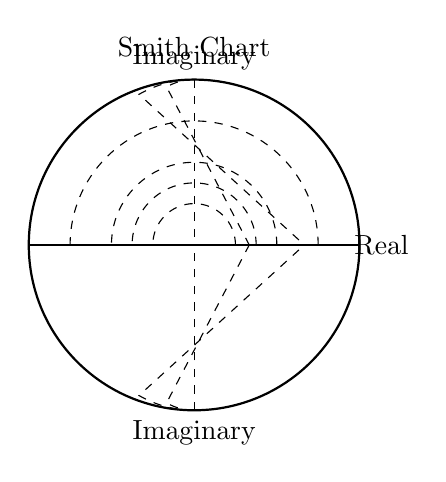
\begin{tikzpicture}[scale=0.7]
    % Draw the Smith chart circle
    \draw[thick] (0,0) circle (3);
    
    % Draw a horizontal line for the resistance
    \draw[thick] (-3,0) -- (3,0);
    
    % Draw sample resistance circles
    \foreach \r in {0.5,0.75,1,1.5,2} {
        \draw[dashed] ({\r*3/2},0) arc (0:180:3*\r/2);
    }

    % Draw sample reactance arcs
    \foreach \x in {-1,-2,-3} {
        \draw[dashed] (0,3) arc (90:120:3+\x) -- (3+\x,0);
        \draw[dashed] (0,-3) arc (-90:-120:3+\x) -- (3+\x,0);
    }
    
    % Label the axes
    \node at (3.4,0) {Real};
    \node at (0,3.4) {Imaginary};
    \node at (0,-3.4) {Imaginary};
    
    % Add a title
    \node at (0,3.6) {Smith Chart};
\end{tikzpicture}

Understanding these concepts will arm the engineer with the knowledge necessary to navigate the complexities of RF design and application effectively.
